% 48 x 36 inch poster. Compile with pdfLaTeX.
% Every figure is a PDF written by make_figs.py from docs/data.js, the same values the
% project page plots, so the poster and the page cannot disagree.
\documentclass{article}
\usepackage[paperwidth=48in,paperheight=36in,margin=0pt]{geometry}
\usepackage[T1]{fontenc}
\usepackage{amsmath,amssymb}
\usepackage{libertine}
\usepackage{graphicx,xcolor,tikz}
\usepackage[skins]{tcolorbox}
\usepackage{qrcode,microtype}
\usepackage[hidelinks]{hyperref}
\graphicspath{{figs/}}
\pagestyle{empty}
\definecolor{yale}{HTML}{00356B}
\definecolor{ink}{HTML}{202A35}
\definecolor{muted}{HTML}{536272}
\definecolor{wash}{HTML}{EDF3F8}
\definecolor{rulegray}{HTML}{D3DEE7}
\newcommand{\bodytype}{\fontsize{39}{50}\selectfont}
\newcommand{\captiontype}{\fontsize{28}{36}\selectfont}
\newcommand{\colsetup}{\bodytype\raggedright\setlength{\parindent}{0pt}\setlength{\parskip}{0.26in}\setlength{\abovedisplayskip}{0.16in}\setlength{\belowdisplayskip}{0.16in}}
\newcommand{\heading}[2]{{\fontsize{46}{56}\selectfont\bfseries\color{yale}#1\quad #2\par}\vspace{0.16in}}
\newcommand{\subhead}[1]{{\fontsize{36}{45}\selectfont\bfseries\color{yale}#1\par}\vspace{0.06in}}
\newcommand{\figcaption}[1]{{\captiontype\color{muted}#1\par}}
\newtcolorbox{finding}[1][]{enhanced,colback=wash,colframe=wash,boxrule=0pt,arc=0pt,
  borderline west={4pt}{0pt}{yale},left=0.26in,right=0.24in,top=0.20in,bottom=0.20in,
  before skip=0.12in,after skip=0.12in,fontupper=\fontsize{35}{45}\selectfont\raggedright,#1}
\newtcolorbox{derivation}{enhanced,colback=white,colframe=rulegray,boxrule=1.2pt,arc=0pt,
  left=0.26in,right=0.26in,top=0.22in,bottom=0.22in,before skip=0.16in,after skip=0.20in,
  fontupper=\fontsize{35}{45}\selectfont\raggedright}
\begin{document}
\null
\begin{tikzpicture}[remember picture,overlay]
\fill[white] (current page.south west) rectangle (current page.north east);

% ---------------------------------------------------------------- header
\node[anchor=north,inner sep=0pt] at ([yshift=-1.5in]current page.north) {\begin{minipage}{40in}\centering
  {\fontsize{88}{98}\selectfont\color{yale}Deduce the World: How Far Can Reasoning Go?\par}
  \vspace{0.36in}
  {\fontsize{48}{58}\selectfont Jeffrey Wei\textsuperscript{1}\qquad Brian Cheung\textsuperscript{2}\par}
  \vspace{0.18in}
  {\fontsize{34}{42}\selectfont\color{muted}\textsuperscript{1}Yale University \qquad \textsuperscript{2}University of California, San Francisco\par}
\end{minipage}};
\node[anchor=north east,inner sep=0pt] at ([xshift=-1.2in,yshift=-1.5in]current page.north east) {\begin{minipage}{3.0in}\centering
{\fontsize{26}{34}\selectfont
\qrcode[height=2.3in]{https://jwei302.github.io/reasoning/}\\[0.14in]
Results \& figures}
\end{minipage}};

% ================================================================ column 1
\node[anchor=north west,inner sep=0pt] at ([xshift=0.9in,yshift=-6.4in]current page.north west) {\begin{minipage}{14.6in}
\colsetup
\heading{1}{Theories, not fitted predictors}

Science deduces the world from first principles, revising its theories where their predictions fail. Deep learning does not. It fits a predictor to existing data, which binds it to that distribution.

We ask whether a reasoning model can form scientific theories, and whether those theories generalize better than deep learning.

{\centering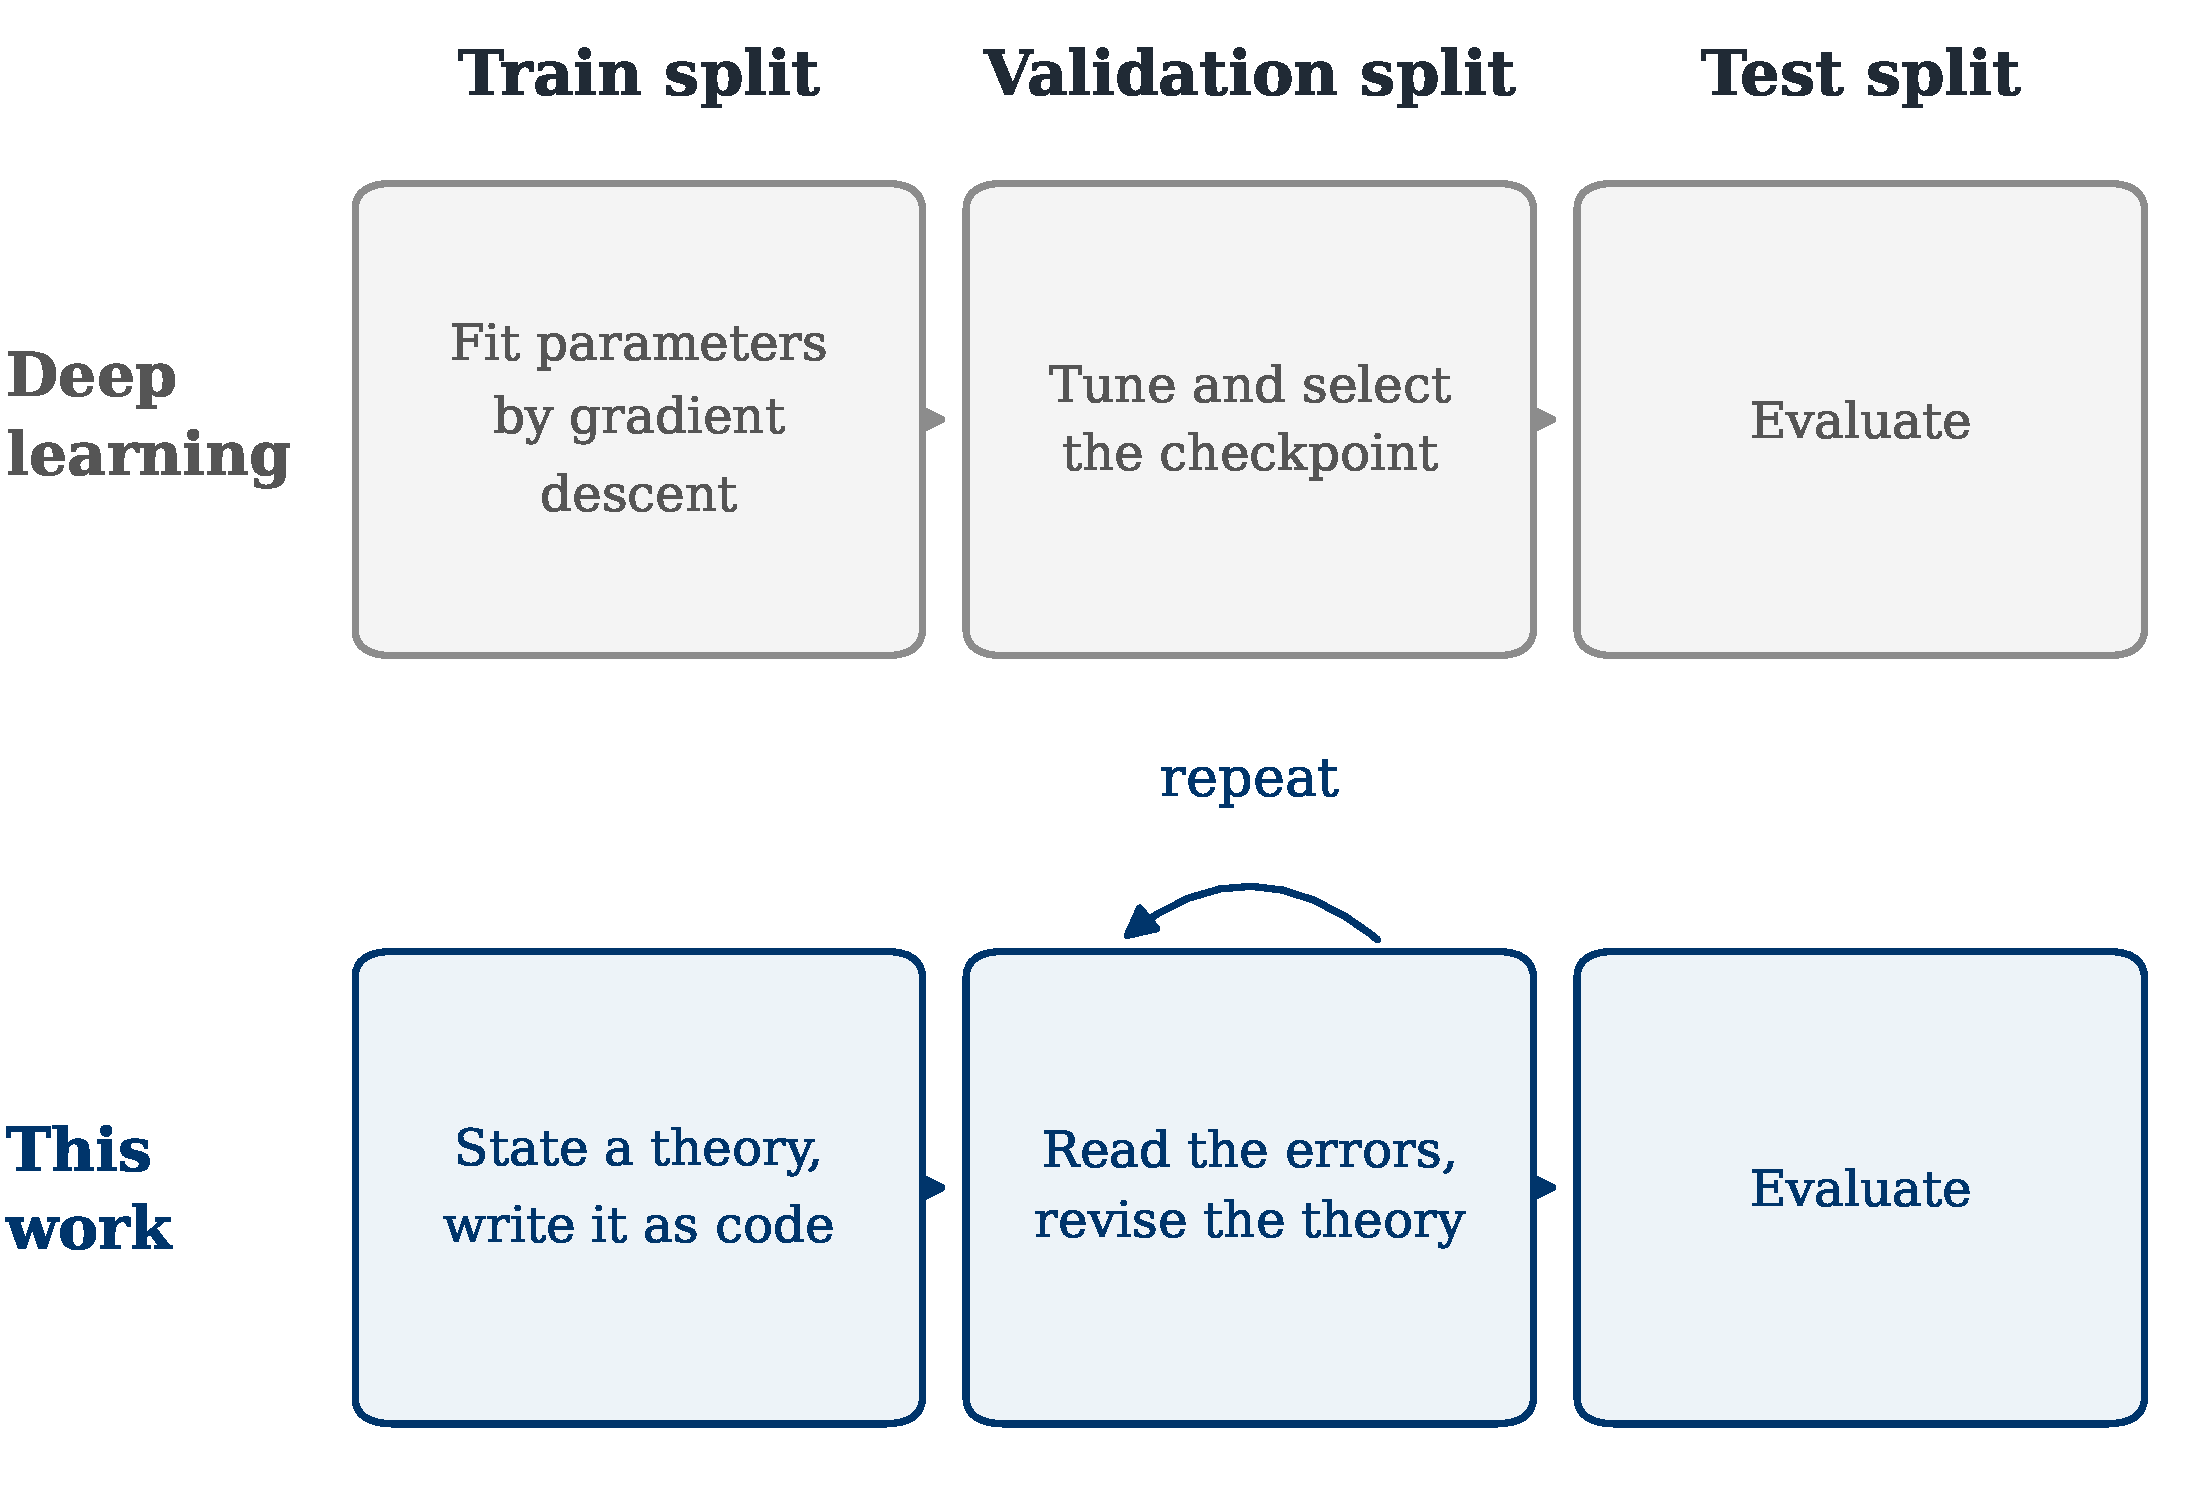
\includegraphics[width=\linewidth]{poster_framework}\par}
\figcaption{We keep the splits of deep learning and replace the learner. The model states a theory, writes it as code, and revises it against validation.}

\vspace{0.10in}
{\captiontype
\begin{tabular}{@{}p{2.5in}p{11.7in}@{}}
\textbf{May} & read papers and the web, measure the training data, inspect its own errors\\[0.08in]
\textbf{May not} & fit parameters to labels, search automatically over rules, store examples, see the test split\\
\end{tabular}\par}

\vspace{0.30in}
\subhead{Reasoning as initialization}
A written theory is also a starting point. Training from written weights converges sooner, and by more as reasoning grows.

{\centering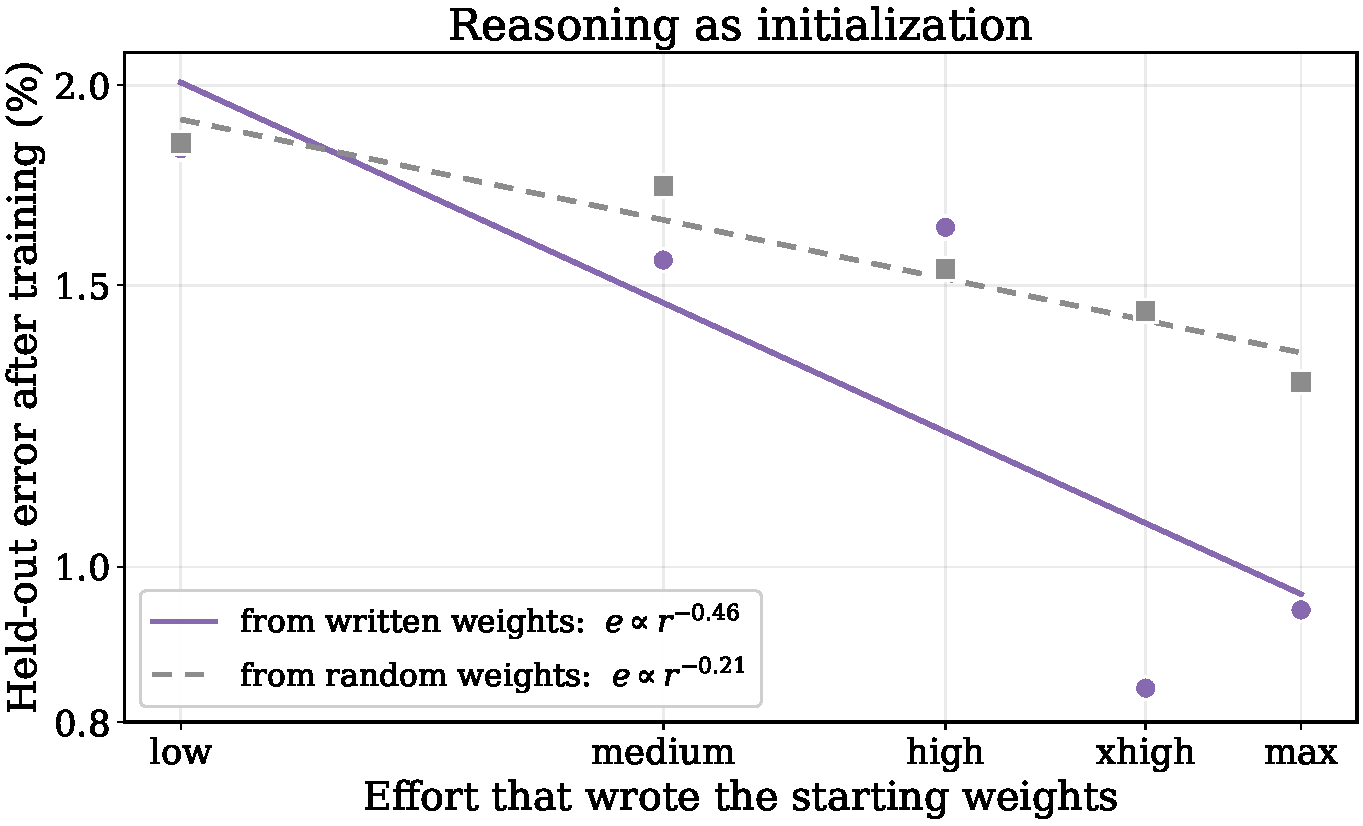
\includegraphics[width=0.80\linewidth]{poster_powerlaw}\par}
\figcaption{Held-out error after a fixed training budget against effort rank, both axes logarithmic.}
\end{minipage}};

% ================================================================ column 2
\node[anchor=north west,inner sep=0pt] at ([xshift=16.6in,yshift=-6.4in]current page.north west) {\begin{minipage}{14.6in}
\colsetup
\heading{2}{How much data a theory needs}

{\centering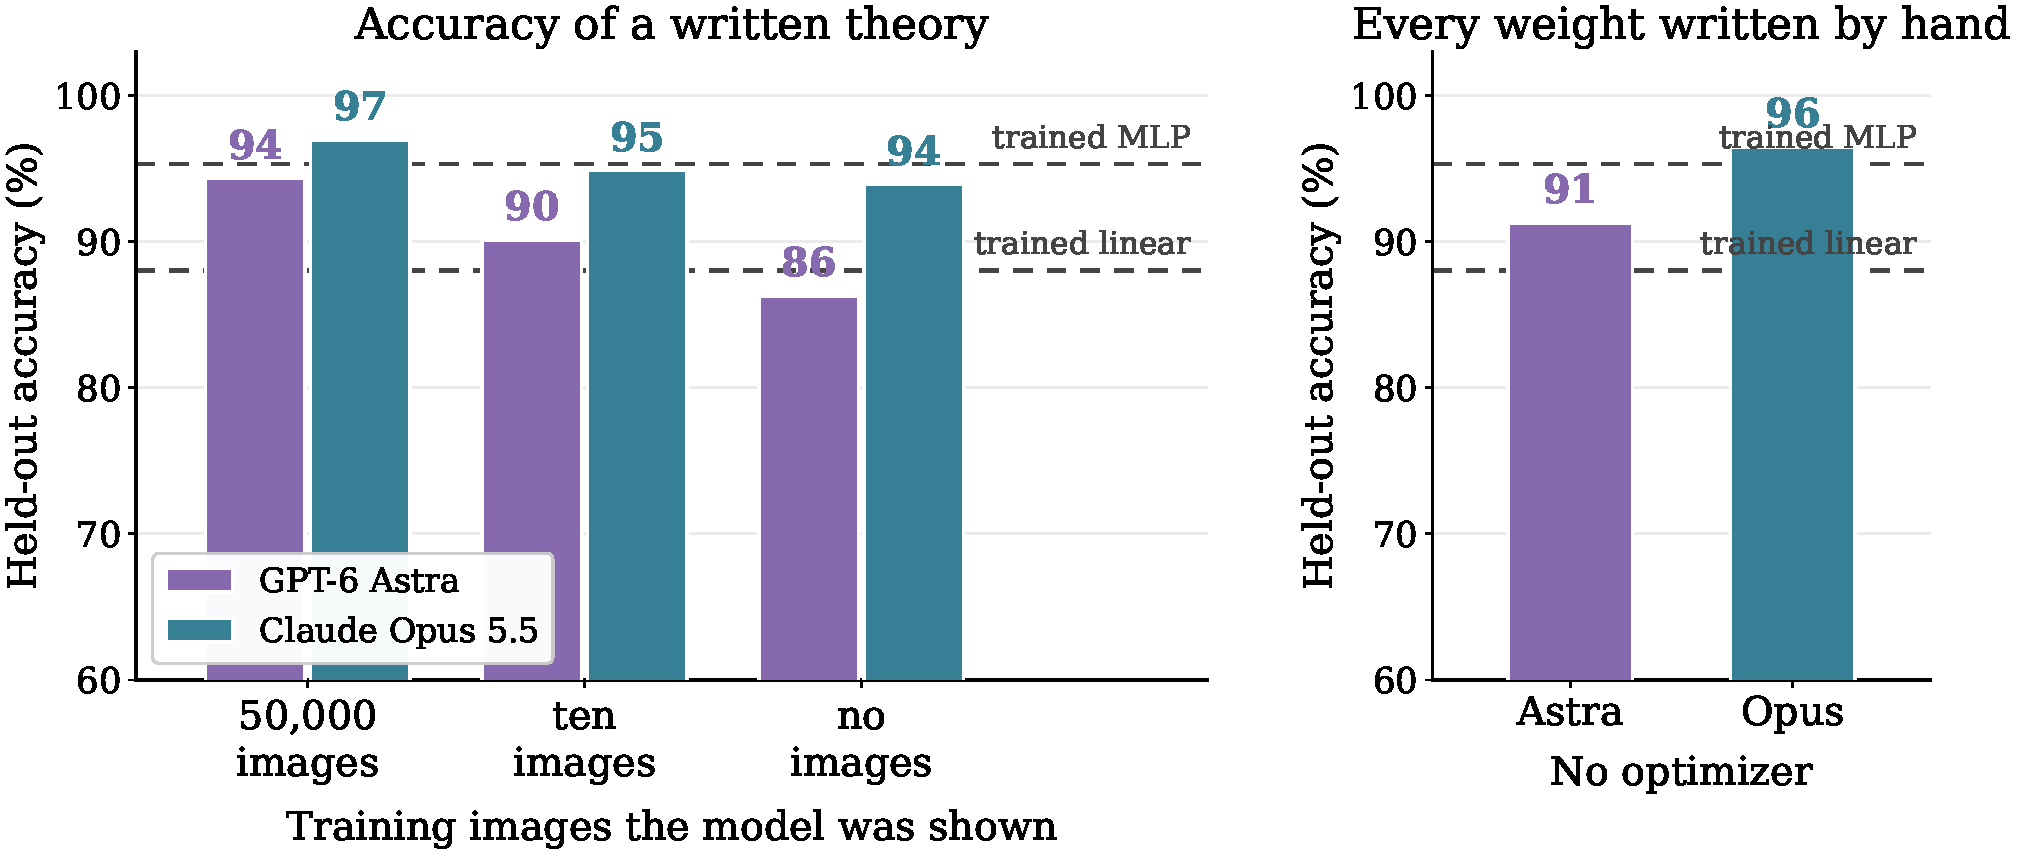
\includegraphics[width=\linewidth]{poster_digits}\par}
\figcaption{Handwritten digits. Best of five reasoning efforts. Dashed lines are trained models on the same split.}

\begin{finding}
Given no training images at all, a theory of how digits are written classifies most of them.
\end{finding}

\vspace{0.26in}
\heading{3}{The same protocol, ten fields}

{\centering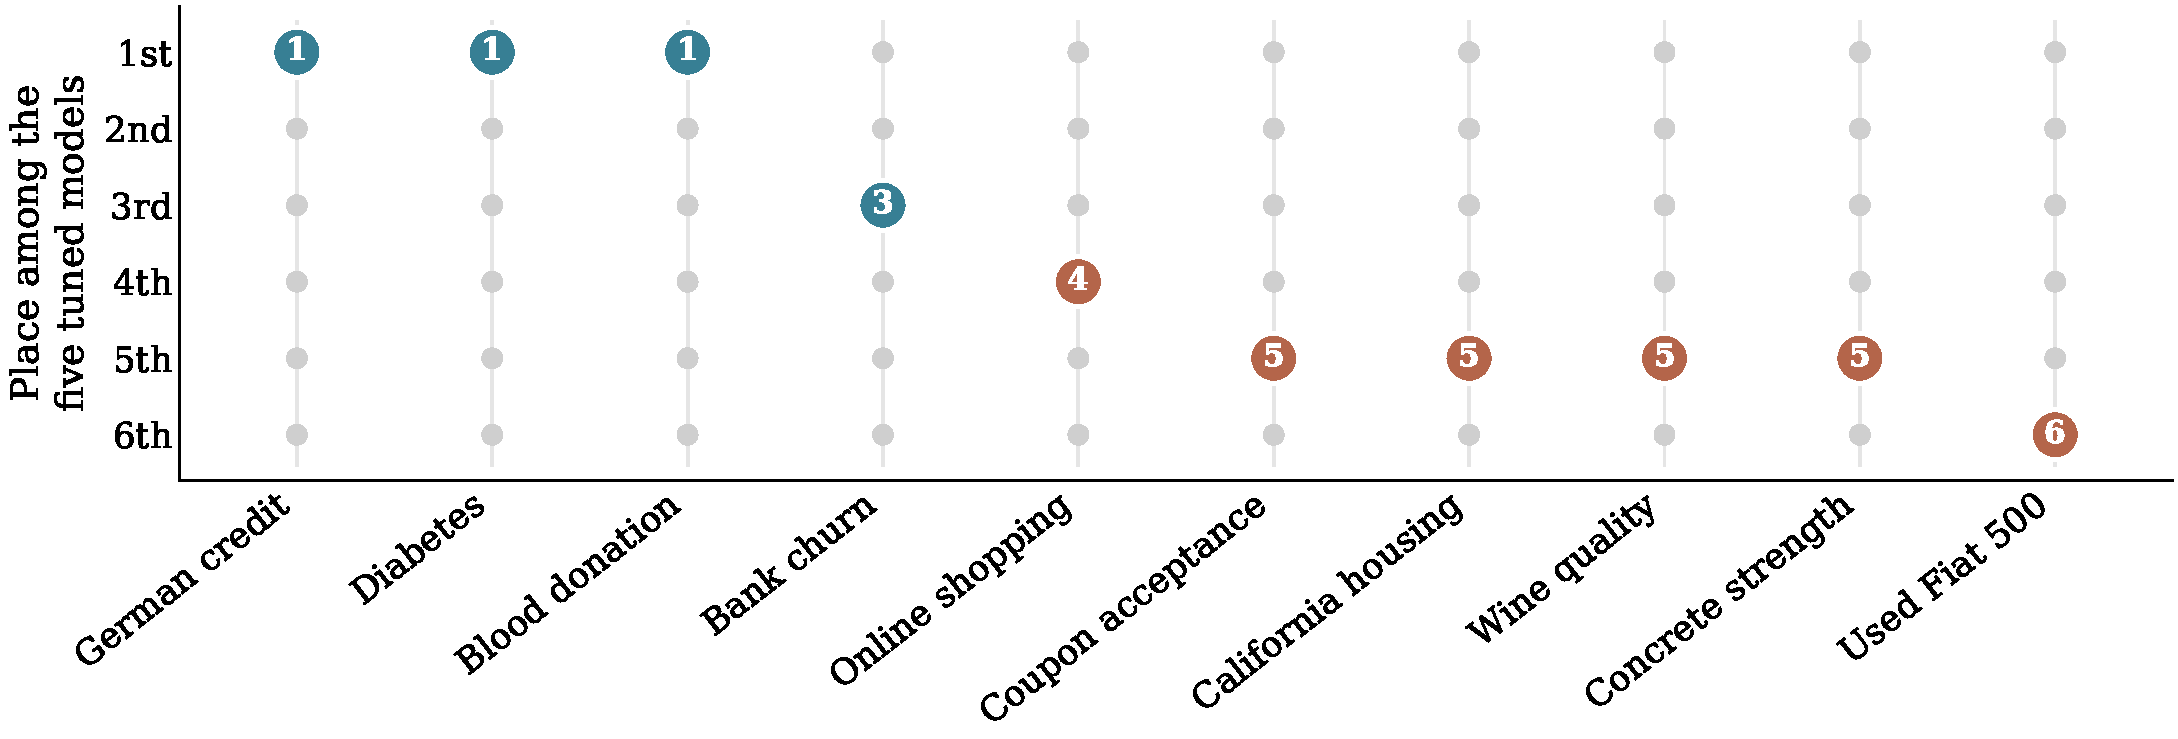
\includegraphics[width=\linewidth]{poster_tabular}\par}
\figcaption{Each task ranks the reasoned theory against linear models, random forests, XGBoost, CatBoost and an MLP, all tuned on the same rows.}

\begin{finding}
Reasoned theories win on small clinical and credit tables, and trail boosted trees where the signal lies in feature interactions.
\end{finding}

\vspace{0.22in}
\begin{derivation}
\subhead{What a theory looks like}
{\captiontype Selected rules from one program on German credit. The points are judgments stated before measurement, not fitted odds ratios.\par}
\vspace{0.14in}
{\fontsize{31}{40}\selectfont
\begin{tabular}{@{}p{4.2in}p{8.8in}@{}}
Checking account & none $+3$, at least 200 DM $+1$, negative $-2$\\[0.06in]
Credit history & critical account elsewhere $+2$, past delay $-1$\\[0.06in]
Loan duration & $-1$ for each twelve months beyond the first twelve\\[0.06in]
Employment & under a year $-1$, four years or more $+1$\\[0.10in]
Output & $P(\text{good}) = 1/(1+e^{-(\text{score}-1)/2})$\\
\end{tabular}\par}
\end{derivation}
\end{minipage}};

% ================================================================ column 3
\node[anchor=north west,inner sep=0pt] at ([xshift=32.3in,yshift=-6.4in]current page.north west) {\begin{minipage}{14.6in}
\colsetup
\heading{4}{Deriving a scientific score}

A structure predictor returns a complex and an estimate of its own error. Each session receives that matrix and nothing else.

{\centering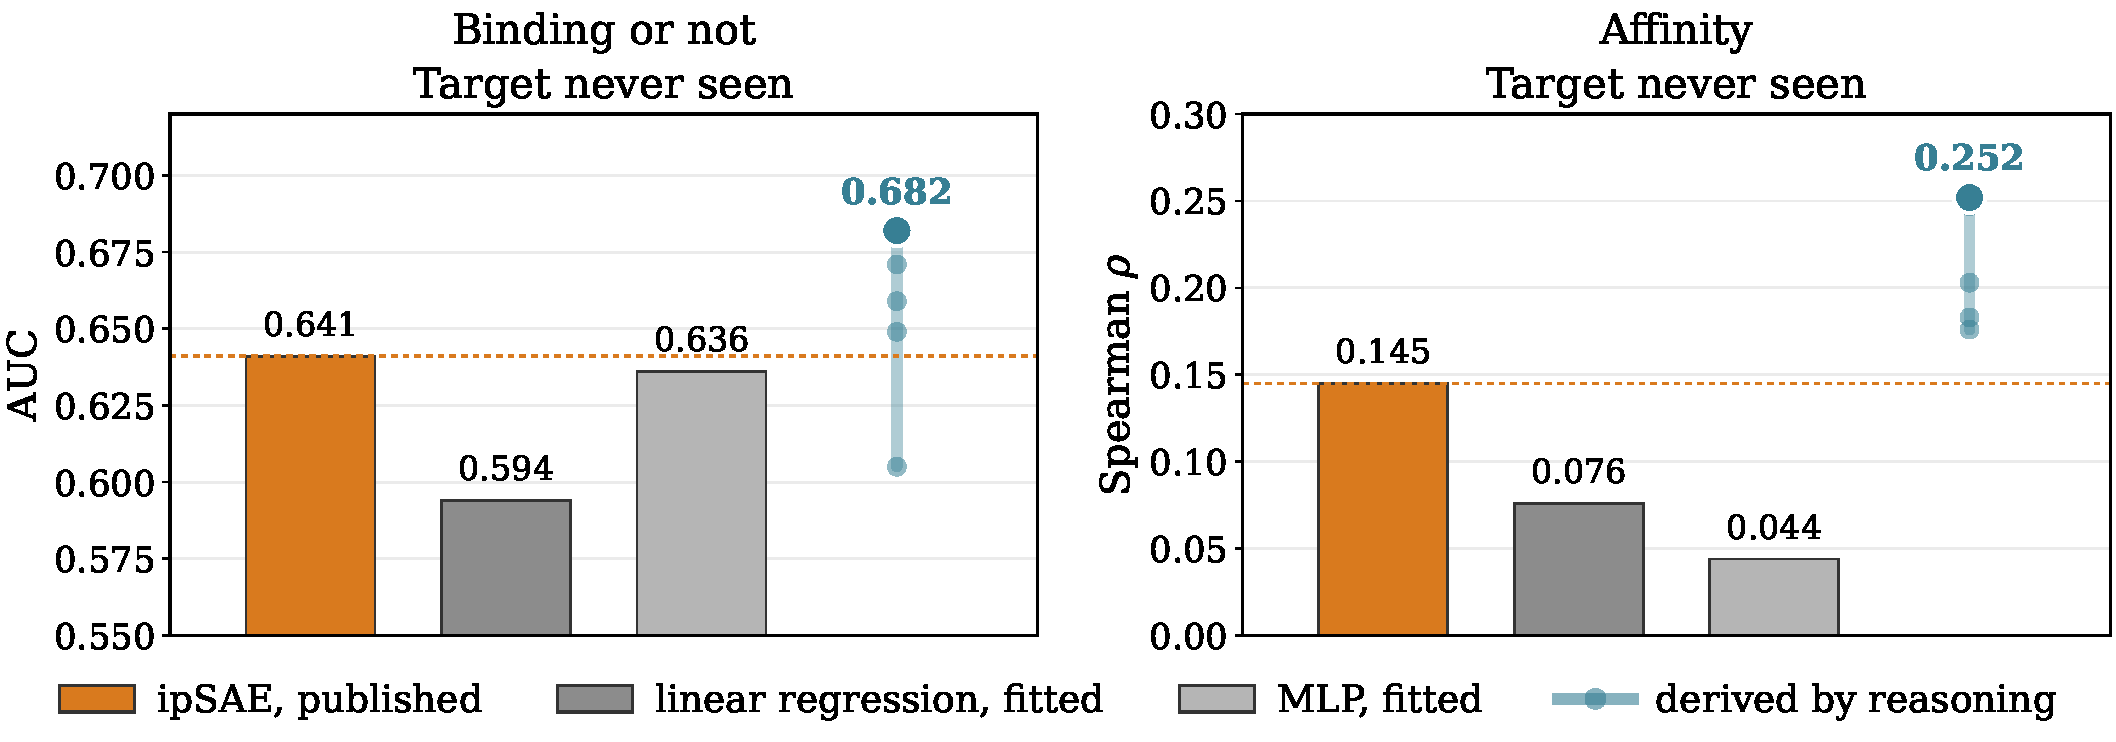
\includegraphics[width=\linewidth]{poster_ipsae}\par}
\figcaption{704 designed binders against five targets. The middle and right panels hold out an entire target.}

\begin{derivation}
\subhead{Derived, not fitted}
Treating the bound complex as a harmonic well, with $\sigma_{\text{iface}}$ the precision of the interface and $\sigma_0$ the precision the binder achieves within itself,
{\fontsize{34}{42}\selectfont
\[
\kappa=\Big(\frac{\sigma_0}{\sigma_{\text{iface}}}\Big)^{2},\qquad
\mathrm{p}K_\mathrm{d}=\mathrm{p}K_\mathrm{d,ref}+3\log_{10}\kappa .
\]}
The 3 is half the six rigid-body degrees of freedom that association confines. Nothing is fitted.
\end{derivation}

{\centering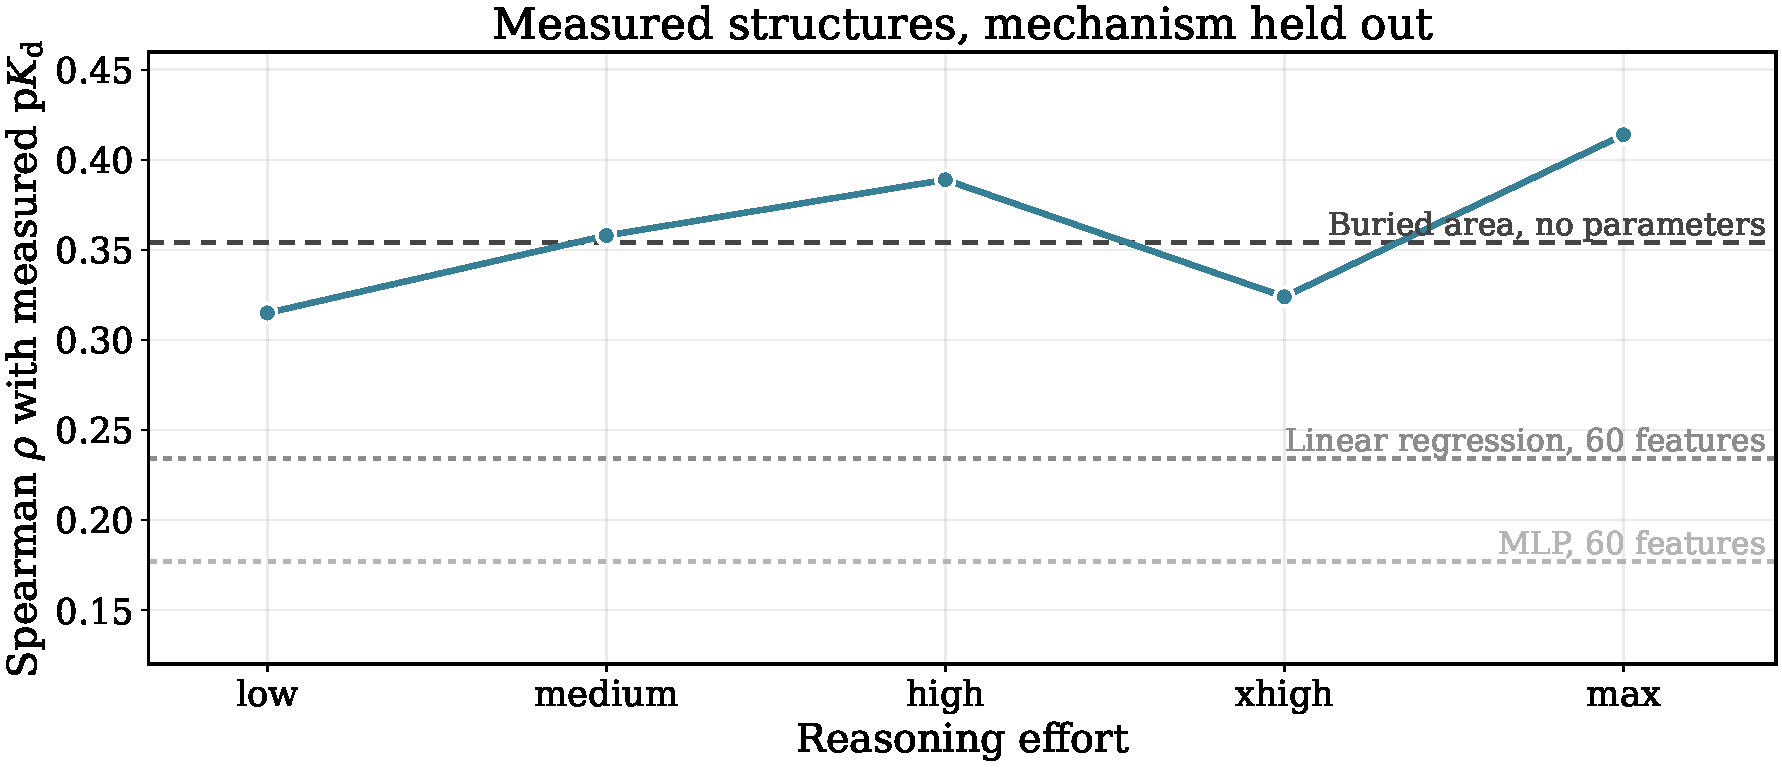
\includegraphics[width=0.96\linewidth]{poster_skempi}\par}
\figcaption{Measured structures grouped by mechanism of association. One mechanism is held out whole.}

\begin{finding}
What transfers is a dimensionless ratio the pair supplies itself. What fails is anything calibrated on the cases it was fitted to.
\end{finding}
\end{minipage}};

% ---------------------------------------------------------------- footer
\node[anchor=south,inner sep=0pt] at ([yshift=0.70in]current page.south) {\begin{minipage}{46in}\centering
{\fontsize{25}{32}\selectfont\color{muted}
Caveats: these models have read the literature of every domain we test, so recall and derivation are not fully separable. The protein cohort is curated candidates rather than a random draw, held-out counts are small and nothing is bootstrapped. An effort setting is not a measure of compute. Frozen protocols, programs and research logs are kept for every run.\par}
\end{minipage}};

\end{tikzpicture}
\end{document}
